
\section{Tabular Data Structure}
This package provides an object-oriented tabular datatype in Tcl, building upon the type system framework provided by the \textcolor{blue}{\href{https://github.com/ambaker1/vutil}{vutil}} package.

The string representation of this datatype is a dictionary, with keys representing the table header, and values representing the table columns.
The values in the first column must be unique, and are called the table ``keys''. 
Correspondingly, the first header entry is called the ``keyname''. 
The remaining header entries are called the table ``fields'', and the remaining columns are the data stored in the table.
The conceptual layout of the table is illustrated in the figure below.
\vspace{\baselineskip}
\FloatBarrier
\begin{figure}[!htb]
    \centering
    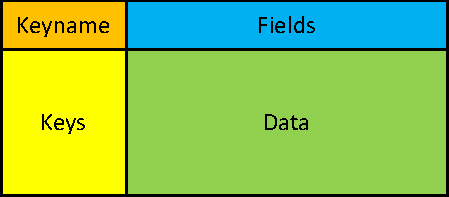
\includegraphics{figures/table.pdf}
    \caption{Conceptual Representation of Tabular Data Structure}
    \label{fig:table_props}
\end{figure}
There is no restriction on the type of data that can be stored in a table, as shown in the example below, which has keyname ``key'', keys ``1 2 3'' and fields ``A B''.
Note that missing values are represented by blanks. 
\begin{example}{String representation of tabular data type}
\begin{lstlisting}
key {1 2 3} A {5.6 {} 2.22} B {{hello world} 4.5 foo}
\end{lstlisting}
\end{example}

\clearpage
\section{Creating Table Objects}
This package provides the ``table'' type class, using the type system provided by the ``vutil'' package. 
The command \cmdlink{table} creates a new table object variable, which uses the class \texttt{::taboo::tblobj}.
\begin{syntax}
\command{table} \$refName <\$value>
\end{syntax}
\begin{args}
\$refName & Reference name to tie object to. \\
\$value & Value of table. Default blank.
\end{args}

Below is the example table used in the remainder of the documentation examples.
Note that this format is also compatible with the string representation of Tcl arrays and dictionaries.
\begin{example}{Example table}
\begin{lstlisting}
table tableObj {
    key {1 2 3 4 5} 
    x {3.44 4.61 8.25 5.20 3.26}
    y {7.11 1.81 7.56 6.78 9.92}
    z {8.67 7.63 3.84 1.11 4.56}
}
puts [$tableObj]
\end{lstlisting}
\tcblower
\begin{lstlisting}
key {1 2 3 4 5} x {3.44 4.61 8.25 5.20 3.26} y {7.11 1.81 7.56 6.78 9.92} z {8.67 7.63 3.84 1.11 4.56}
\end{lstlisting}
\end{example}

\subsection{Wiping, Clearing, and Cleaning a Table}
The method \methodlink[0]{table}{wipe} removes all data from a table object, so that its state is the same as a fresh table.
The method \methodlink[0]{table}{clear} only removes the data and keys stored in the table, keeping the fields and other metadata.
The method \methodlink[0]{table}{clean} only removes keys and fields that have no data.
\begin{syntax}
\method{table}{wipe}
\end{syntax}
\begin{syntax}
\method{table}{clear}
\end{syntax}
\begin{syntax}
\method{table}{clean}
\end{syntax}


\clearpage
\subsection{Standard Methods}
Because the table objects are object variables, they have the same basic methods provided by the ``vutil'' package.
For more info on these methods, see the documentation for the ``vutil'' package.
\begin{syntax}
\method{table}{-{}->} \$refName \\
\method{table}{<-} \$object \\
\method{table}{=} \$value \\
\method{table}{::=} \$body \\
\method{table}{info} <\$field> \\
\method{table}{print} <-nonewline> <\$channelID> \\
\method{table}{destroy}
\end{syntax}
\begin{args}
\$refName & Reference name to copy to. \\
\$object & Table object. \\
\$value & Table value to assign. \\
\$body & Tcl script to evaluate and set as table value. \\
\$field & Field to query (fields ``height'' and ``width'' added). \\
\$channelID & Open channel to print to. 
\end{args}
Note that the methods \texttt{.=} and \texttt{:=} are also available, but they are not recommended for tables.
Also note that ``taboo'' tables are always initialized, so the ``exists'' field of the object variable will always be true.

\begin{example}{Copying a table}
\begin{lstlisting}
$tableObj --> tableCopy
puts [$tableCopy info]
\end{lstlisting}
\tcblower
\begin{lstlisting}
exists 1 height 5 type table value {key {1 2 3 4 5} x {3.44 4.61 8.25 5.20 3.26} y {7.11 1.81 7.56 6.78 9.92} z {8.67 7.63 3.84 1.11 4.56}} width 3
\end{lstlisting}
\end{example}
\clearpage

\subsection{Get/Set Keyname}
The keyname of a table can be accessed or modified directly with their respective methods. 
\begin{syntax}
\method{table}{keyname} <\$keyname>
\end{syntax}
\begin{args}
\$keyname & Header for table keys. Default blank to return current name.
\end{args}
\subsection{Get Keys and Fields}
The table keys and fields are ordered lists of the row and column names of the table.
They can be queried with the methods \methodlink[0]{table}{keys} and \methodlink[0]{table}{fields}, respectively. 
\begin{syntax}
\method{table}{keys} <\$index>
\end{syntax}
\begin{syntax}
\method{table}{fields} <\$index>
\end{syntax}
\begin{args}
\$index & Index arguments, using ``ndlist'' index notation. \\
& Default ``\texttt{:}`` for all keys/fields.
\end{args}
\subsection{Table Dimensions}
The number of keys can be queried with \methodlink{table}{height} and the number of fields can be queried with \methodlink{table}{width}. 
These are also properties accessible with the standard method \methodlink[0]{table}{info}.
Note that rows and columns with missing data will be counted.
\begin{syntax}
\method{table}{height}
\end{syntax}
\begin{syntax}
\method{table}{width}
\end{syntax}

\begin{example}{Accessing table keys and table dimensions}
\begin{lstlisting}
puts [$tableObj keys]
puts [$tableObj keys 0:end-1]
puts [$tableObj height]
\end{lstlisting}
\tcblower
\begin{lstlisting}
1 2 3 4 5
1 2 3 4
5
\end{lstlisting}
\end{example}
\clearpage
\subsection{Get Table Data (Dictionary Form)}
The method \methodlink[0]{table}{data} returns the table data in unsorted dictionary form, where blanks are represented by missing dictionary entries. 
\begin{syntax}
\method{table}{data} <\$key>
\end{syntax}
\begin{args}
\$key & Key to get row dictionary from (default returns all rows). 
\end{args}

\subsection{Get Table Data (Matrix Form)}
The method \methodlink[0]{table}{values} returns a matrix (list of rows) that represents the data in the table, where the rows correspond to the keys and the columns correspond to the fields. Missing entries are represented by blanks in the matrix unless specified otherwise.
\begin{syntax}
\method{table}{values} <\$filler>
\end{syntax}
\begin{args}
\$filler & Filler for missing values, default blank.
\end{args}
\begin{example}{Getting table data in dictionary and matrix form}
\begin{lstlisting}
puts [$tableObj data]
puts [$tableObj data 3]
puts [$tableObj values]
\end{lstlisting}
\tcblower
\begin{lstlisting}
1 {x 3.44 y 7.11 z 8.67} 2 {x 4.61 y 1.81 z 7.63} 3 {x 8.25 y 7.56 z 3.84} 4 {x 5.20 y 6.78 z 1.11} 5 {x 3.26 y 9.92 z 4.56}
x 8.25 y 7.56 z 3.84
{3.44 7.11 8.67} {4.61 1.81 7.63} {8.25 7.56 3.84} {5.20 6.78 1.11} {3.26 9.92 4.56}
\end{lstlisting}
\end{example}
\clearpage
\subsection{Check Existence of Table Keys/Fields}
The existence of a table key, field, or table value can be queried with the method \methodlink[0]{table}{exists}. 
\begin{syntax}
\method{table}{exists} key \$key \\
\$tableObj exists field \$field \\
\$tableObj exists value \$key \$field
\end{syntax}
\begin{args}
\$key & Key to check. \\
\$field & Field to check.
\end{args}
\subsection{Get Row/Column Indices}
The row or column index of a table key or field can be queried with the method \methodlink[0]{table}{find}. 
If the key or field does not exist, returns an error.

\begin{syntax}
\method{table}{find} key \$key \\
\$tableObj find field \$field
\end{syntax}
\begin{args}
\$key & Key to find. \\
\$field & Field to find.
\end{args}

\begin{example}{Find column index of a field}
\begin{lstlisting}
puts [$tableObj exists field z]
puts [$tableObj find field z]
\end{lstlisting}
\tcblower
\begin{lstlisting}
1
2
\end{lstlisting}
\end{example}

\clearpage
\section{Table Entry and Access}
Data entry and access to a table object can be done with single values with the methods \methodlink[0]{table}{set} and \methodlink[0]{table}{get}, entire rows with \methodlink[0]{table}{rset} and \methodlink[0]{table}{rget}, entire columns with \methodlink[0]{table}{cset} and \methodlink[0]{table}{cget}, or in matrix fashion with \methodlink[0]{table}{mset} and \methodlink[0]{table}{mget}. 
If entry keys/fields do not exist, they are added to the table. 
Additionally, since blank values represent missing data, setting a value to blank effectively unsets the table entry, but does not remove the key or field. 
\subsection{Single Value Entry and Access}
The methods \methodlink[0]{table}{set} and \methodlink[0]{table}{get} allow for easy entry and access of single values in the table. 
Note that multiple field-value pairings can be used in \methodlink{table}{set}. 
\begin{syntax}
\method{table}{set} \$key \$field \$value ...
\end{syntax}
\begin{syntax}
\method{table}{get} \$key \$field <\$filler>
\end{syntax}
\begin{args}
\$key & Key of row to set/get data in/from. \\
\$field & Field of column to set/get data in/from. \\
\$value & Value to set. \\
\$filler & Filler to return if value is missing. Default blank. 
\end{args}

\begin{example}{Setting multiple values}
\begin{lstlisting}
$tableObj --> tableCopy
$tableCopy set 1 x 2.00 y 5.00 foo bar
puts [$tableCopy data 1]
\end{lstlisting}
\tcblower
\begin{lstlisting}
x 2.00 y 5.00 z 8.67 foo bar
\end{lstlisting}
\end{example}
\clearpage
\subsection{Row Entry and Access}
The methods \methodlink[0]{table}{rset} and \methodlink[0]{table}{rget} allow for easy row entry and access.
Entry list length must match table width or be scalar.
If entry list is blank, it will delete the row, but not the key.
\begin{syntax}
\method{table}{rset} \$key \$row
\end{syntax}
\begin{syntax}
\method{table}{rget} \$key <\$filler>
\end{syntax}
\begin{args}
\$key & Key of row to set/get. \\
\$row & List of values (or scalar) to set. \\
\$filler & Filler for missing values. Default blank. 
\end{args}
\subsection{Column Entry and Access}
The methods \methodlink[0]{table}{cset} and \methodlink[0]{table}{cget} allow for easy column entry and access.
Entry list length must match table height or be scalar.
If entry list is blank, it will delete the column, but not the field.
\begin{syntax}
\method{table}{cset} \$field \$column
\end{syntax}
\begin{syntax}
\method{table}{cget} \$field <\$filler>
\end{syntax}
\begin{args}
\$field & Field of column to set/get. \\
\$column & List of values (or scalar) to set. \\
\$filler & Filler for missing values. Default blank. 
\end{args}
\clearpage
\subsection{Matrix Entry and Access}
The methods \methodlink[0]{table}{mset} and \methodlink[0]{table}{mget} allow for easy matrix-style entry and access.
Entry matrix size must match table size or be scalar.
\begin{syntax}
\method{table}{mset} \$keys \$fields \$matrix 
\end{syntax}
\begin{syntax}
\method{table}{mget} \$keys \$fields <\$filler>
\end{syntax}
\begin{args}
\$keys & List of keys to set/get (default all keys). \\
\$fields & List of keys to set/get (default all keys). \\
\$matrix & Matrix of values (or scalar) to set. \\
\$filler & Filler for missing values. Default blank. 
\end{args}

Below is an example of how you can construct a table from scratch. Note also how you can create a table using the ``vutil'' command \textit{new} instead of the command \cmdlink{table}.
\begin{example}{Matrix entry and access}
\begin{lstlisting}
::vutil::new table T
$T add keys 1 2 3 4
$T add fields A B
$T mset [$T keys] [$T fields] 0.0; # Initialize as zero
$T mset [$T keys 0:2] A {1.0 2.0 3.0}; # Set subset of table
puts [$T values]
\end{lstlisting}
\tcblower
\begin{lstlisting}
{1.0 0.0} {2.0 0.0} {3.0 0.0} {0.0 0.0}
\end{lstlisting}
\end{example}

\clearpage

\section{Iterating Over Table Data}
Table data can be looped through, row-wise, with the method \methodlink[0]{table}{with}. 
Variables representing the key values and fields will be assigned their corresponding values, with blanks representing missing data. 
The variable representing the key (table keyname) is static, but changes made to field variables are reflected in the table. 
Unsetting a field variable or setting its value to blank unsets the corresponding data in the table. 
\begin{syntax}
\method{table}{with} \$body
\end{syntax}
\begin{args}
\$body & Code to execute.
\end{args}
\begin{example}{Iterating over a table, accessing and modifying field values}
\begin{lstlisting}
$tableObj --> tableCopy
set a 20.0
$tableCopy add fields q
$tableCopy with {
    puts [list $key $x]; # access key and field value
    set q [expr {$x*2 + $a}]; # modify field value
}
puts [$tableCopy cget q]
\end{lstlisting}
\tcblower
\begin{lstlisting}
1 3.44
2 4.61
3 8.25
4 5.20
5 3.26
26.88 29.22 36.5 30.4 26.52
\end{lstlisting}
\end{example}
Note: Just like in \textit{dict with}, the key variable and field variables in \methodlink{table}{with} persist after the loop.
\clearpage
\section{Field Expressions}
The method \methodlink[0]{table}{expr} computes a list of values according to a field expression. 
In the same style as referring to variables with the dollar sign (\$), the ``at'' symbol (@) is used by \methodlink{table}{expr} to refer to field values, or row keys if the keyname is used. 
If any referenced fields have missing values for a table row, the corresponding result will be blank as well. 
The resulting list corresponds to the keys in the table.
\begin{syntax}
\method{table}{expr} \$fieldExpr
\end{syntax}
\begin{args}
\$fieldExpr & Field expression.
\end{args}
\subsection{Editing Table Fields}
Field expressions can be used to edit existing fields or add new fields in a table with the method \methodlink[0]{table}{fedit}. 
If any of the referenced fields are blank, the corresponding entry will be blank as well.
\begin{syntax}
\method{table}{fedit} \$field \$fieldExpr
\end{syntax}
\begin{args}
\$field & Field to set. \\
\$fieldExpr & Field expression.
\end{args}
\begin{example}{Using field expressions}
\begin{lstlisting}
$tableObj --> tableCopy
set a 20.0
puts [$tableCopy cget x]
puts [$tableCopy expr {@x*2 + $a}]
$tableCopy fedit q {@x*2 + $a}
puts [$tableCopy cget q]
\end{lstlisting}
\tcblower
\begin{lstlisting}
3.44 4.61 8.25 5.20 3.26
26.88 29.22 36.5 30.4 26.52
26.88 29.22 36.5 30.4 26.52
\end{lstlisting}
\end{example}
\clearpage
\subsection{Querying Keys that Match Criteria}
The method \methodlink[0]{table}{filter} returns the keys in a table that match criteria in a field expression.
\begin{syntax}
\method{table}{query} \$fieldExpr
\end{syntax}
\begin{args}
\$fieldExpr & Field expression that results in boolean value (true or false, 1 or 0).
\end{args}
\begin{example}{Getting keys that match criteria}
\begin{lstlisting}
puts [$tableObj query {@x > 3.0 && @y > 7.0}]
\end{lstlisting}
\tcblower
\begin{lstlisting}
1 3 5
\end{lstlisting}
\end{example}

\subsection{Filtering Table Based on Criteria}
The method \methodlink[0]{table}{filter} filters a table to the keys matching criteria in a field expression. 
\begin{syntax}
\method{table}{filter} \$fieldExpr
\end{syntax}
\begin{args}
\$fieldExpr & Field expression that results in boolean value (true or false, 1 or 0).
\end{args}
\begin{example}{Filtering table to only include keys that match criteria}
\begin{lstlisting}
$tableObj --> tableCopy
$tableCopy filter {@x > 3.0 && @y > 7.0}
puts [$tableCopy keys]
\end{lstlisting}
\tcblower
\begin{lstlisting}
1 3 5
\end{lstlisting}
\end{example}

\clearpage

\section{Searching a Table}
Besides searching for specific field expression criteria with \methodlink{table}{query}, keys matching criteria can be found with the method \methodlink[0]{table}{search}. 
The method \methodlink[0]{table}{search} searches a table using the Tcl \textit{lsearch} command on the keys or field values. The default search method uses glob pattern matching, and returns matching keys.
This search behavior can be changed with the various options, which are taken directly from the Tcl \textit{lsearch} command. 
Therefore, while brief descriptions of the options are provided here, they are explained more in depth in the Tcl documentation, with the exception of the -inline option.
The -inline option filters a table based on the search criteria.
\begin{syntax}
\method{table}{search} <\$option ...> <\$field> \$value
\end{syntax}
\begin{args}
\$option ... & Searching options. Valid options: \\
\quad -exact & \quad Compare strings exactly \\
\quad -glob & \quad Use glob-style pattern matching (default) \\
\quad -regexp & \quad Use regular expression matching \\
\quad -sorted & \quad Assume elements are in sorted order \\
\quad -all & \quad Get all matches, rather than the first match \\
\quad -not & \quad Negate the match(es) \\
\quad -ascii & \quad Use string comparison (default) \\
\quad -dictionary & \quad Use dictionary-style comparison \\
\quad -integer & \quad Use integer comparison \\
\quad -real & \quad Use floating-point comparison \\
\quad -nocase & \quad Search in a case-insensitive manner \\
\quad -increasing & \quad Assume increasing order (default) \\
\quad -decreasing & \quad Assume decreasing order \\
\quad -bisect & \quad Perform inexact match \\
\quad -inline & \quad Filter table instead of returning keys. \\
\quad -{}- & \quad Signals end of options \\
\$field  & Field to search. If blank, searches keys. \\
\$value & Value or pattern to search for
\end{args}
Note: If a field contains missing values, they will only be included in the search if the search options allow (e.g. blanks are included for string matching, but not for numerical matching).
\clearpage
\section{Sorting a Table}
The method \methodlink[0]{table}{sort} sorts a table by keys or field values. 
The default sorting method is in increasing order, using string comparison. 
This sorting behavior can be changed with the various options, which are taken directly from the Tcl \textit{lsort} command. 
Therefore, while brief descriptions of the options are provided here, they are explained more in depth in the Tcl documentation.
Note: If a field contains missing values, the missing values will be last, regardless of sorting options. 
\begin{syntax}
\method{table}{sort} <\$option ...> <\$field ...>
\end{syntax}
\begin{args}
\$option ... & Sorting options. Valid options: \\
\quad -ascii & \quad Use string comparison (default) \\
\quad -dictionary & \quad Use dictionary-style comparison \\
\quad -integer & \quad Use integer comparison \\
\quad -real & \quad Use floating comparison \\
\quad -increasing & \quad Sort the list in increasing order (default) \\
\quad -decreasing & \quad Sort the list in decreasing order \\
\quad -nocase & \quad Compare in a case-insensitive manner \\
\quad -{}- & \quad Signals end of options \\
\$field ...  & Fields to sort by (in order of sorting). If blank, sorts by keys.
\end{args}
\begin{example}{Searching and sorting}
\begin{lstlisting}
$tableObj --> tableCopy
puts [$tableCopy search -real x 8.25]; # returns first matching key
$tableCopy sort -real x
puts [$tableCopy keys]
puts [$tableCopy cget x]; # table access reflects sorted keys
puts [$tableCopy search -sorted -bisect -real x 5.0]
\end{lstlisting}
\tcblower
\begin{lstlisting}
3
5 1 2 4 3
3.26 3.44 4.61 5.20 8.25
2
\end{lstlisting}
\end{example}
\clearpage
\section{Merging Tables}
Data from other tables can be merged into the table object with \methodlink{table}{merge}. 
In order to merge, all the tables must have the same keyname and fieldname. 
If the merge is valid, the table data is combined, with later entries taking precedence. 
Additionally, the keys and fields are combined, such that if a key appears in any of the tables, it is in the combined table.

\begin{syntax}
\method{table}{merge} \$object ...
\end{syntax}
\begin{args}
\$object ... & Other table objects to merge into table. Does not destroy the input tables. 
\end{args}

\begin{example}{Merging data from other tables}
\begin{lstlisting}
$tableObj --> tableCopy
table newTable
$newTable set 1 x 5.00 q 6.34
$tableCopy merge $newTable
$tableCopy print
\end{lstlisting}
\tcblower
\begin{lstlisting}
key {1 2 3 4 5} x {5.00 4.61 8.25 5.20 3.26} y {7.11 1.81 7.56 6.78 9.92} z {8.67 7.63 3.84 1.11 4.56} q {6.34 {} {} {} {}}
\end{lstlisting}
\end{example}
\clearpage
\section{Table Manipulation}
The following methods are useful for adding, removing, and rearranging rows and columns in a table.

\subsection{Overwriting Keys/Fields}
The method \methodlink[0]{table}{define} overwrites the keys and fields of the table, filtering the data or adding keys and fields as necessary. 
For example, if the keys are defined to be a subset of the current keys, it will filter the data to only include the key subset. 
\begin{syntax}
\method{table}{define} keys \$keys \\
\$tableObj define fields \$fields
\end{syntax}
\begin{args}
\$keys & Unique list of keys. \\
\$fields & Unique list of fields.
\end{args}

\subsection{Adding or Removing Keys/Fields}
The method \methodlink[0]{table}{add} adds keys or fields to a table, appending to the end of the key/field lists. 
If a key or field already exists it is ignored.
The method  \methodlink[0]{table}{remove} removes keys or fields and their corresponding rows and columns from a table. If a key or field does not exist, it is ignored. 
\begin{syntax}
\method{table}{add} keys \$key ... \\
\$tableObj add fields \$field ...
\end{syntax}
\begin{syntax}
\method{table}{remove} keys \$key ... \\
\$tableObj remove fields \$field ...
\end{syntax}
\begin{args}
\$key ... & Keys to add/remove. \\
\$field ... & Fields to add/remove.
\end{args}
\clearpage


\subsection{Inserting Keys/Fields}
The method  \methodlink[0]{table}{insert} inserts keys or fields at a specific row or column index. 
Input keys or fields must be unique and must not already exist. 
\begin{syntax}
\method{table}{insert} keys \$index \$key ... \\
\$tableObj insert fields \$index \$field ...
\end{syntax}
\begin{args}
\$index & Row/column index to insert at. \\
\$key ... & Keys to insert. \\
\$field ... & Fields to insert.
\end{args}

\subsection{Renaming Keys/Fields}
The method  \methodlink[0]{table}{rename} renames keys or fields. 
Old keys and fields must exist. 
Duplicates are not allowed in old and new key/field lists.

\begin{syntax}
\method{table}{rename} keys \$old \$new \\
\$tableObj rename fields \$old \$new
\end{syntax}
\begin{args}
\$old & Keys/fields to rename. Must exist. \\
\$new & New keys/fields. Must be same length as \$old. 
\end{args}

\begin{example}{Renaming fields}
\begin{lstlisting}
$tableObj --> tableCopy
$tableCopy rename fields [string toupper [$tableCopy fields]]
puts [$tableObj fields]
puts [$tableCopy fields]
\end{lstlisting}
\tcblower
\begin{lstlisting}
x y z
X Y Z
\end{lstlisting}
\end{example}

\clearpage

\subsection{Moving Keys/Fields}
Existing keys and fields can be moved with the method \methodlink[0]{table}{move}.
\begin{syntax}
\method{table}{move} key \$key \$index \\
\$tableObj move field \$field \$index
\end{syntax}
\begin{args}
\$key & Key to move. \\
\$field & Field to move. \\
\$index & Row/column index to move to. \\
\end{args}

\subsection{Swapping Keys/Fields}
Existing keys and fields can be swapped with the method \methodlink[0]{table}{swap}.
To swap the a field column with the key column, use the method \methodlink[0]{table}{mkkey}.

\begin{syntax}
\method{table}{swap} keys \$key1 \$key2 \\
\$tableObj swap fields \$field1 \$field2
\end{syntax}
\begin{args}
\$key1 \$key2 & Keys to swap. \\
\$field1 \$field2 & Fields to swap.
\end{args}

\begin{example}{Swapping table rows}
\begin{lstlisting}
$tableObj --> tableCopy
$tableCopy swap keys 1 4
$tableCopy print
\end{lstlisting}
\tcblower
\begin{lstlisting}
key {4 2 3 1 5} x {5.20 4.61 8.25 3.44 3.26} y {6.78 1.81 7.56 7.11 9.92} z {1.11 7.63 3.84 8.67 4.56}
\end{lstlisting}
\end{example}

\clearpage

\subsection{Making a Field the Key of a Table}
The method \methodlink[0]{table}{mkkey} makes a field the key of a table, and makes the key a field. 
If a field is empty for some keys, those keys will be lost. 
Additionally, if field values repeat, only the last entry for that field value will be included. 
This method is intended to be used with a field that is full and unique, and if the keyname matches a field name, this command will return an error.
\begin{syntax}
\method{table}{mkkey} \$field
\end{syntax}
\begin{args}
\$field & Field to swap with key.
\end{args}

\subsection{Transposing a Table}
The method \methodlink[0]{table}{transpose} transposes the table, making the keys the fields and the fields the keys.
\begin{syntax}
\method{table}{transpose}
\end{syntax}

\begin{example}{Transposing a table}
\begin{lstlisting}
$tableObj --> tableCopy
$tableCopy transpose
$tableCopy print
\end{lstlisting}
\tcblower
\begin{lstlisting}
key {x y z} 1 {3.44 7.11 8.67} 2 {4.61 1.81 7.63} 3 {8.25 7.56 3.84} 4 {5.20 6.78 1.11} 5 {3.26 9.92 4.56}
\end{lstlisting}
\end{example}